\chapter[Neutral MSSM Higgs Search...]{The Search for neutral MSSM Higgs Bosons in the final state:
$\tau^{+}\tau^{-} \rightarrow e \mu + 4\nu$}

%A search for neutral MSSM Higgs bosons with the ATLAS detector at the
%LHC is presented.  This analysis is based on an integrated luminosity of $20.3 ~fb^{-1}$
%of proton-proton collisions at a center-of-mass energy of 8 TeV. 
%
%The analysis focusses on the decay of neutral Higgs bosons into a pair of tau
%leptons, which subsequently decay to an electron, a muon and four
%neutrinos. Furthermore, 
%

This chapter presents the search for the neutral MSSM Higgs bosons decaying in tau pairs
and fully leptonic final state. This search is based on 20.3 $fb^{-1}$ of 8 TeV data 
recorded by ATLAS experiment during 2012 at Large Hadron Collider~(LHC)~\cite{LHC}.
In this analysis two channels are employed by requiring the
presence or absence of a b-tagged jet, this increases the 
sensitivity to the neutral MSSM Higgs boson via
the b-associated and gluon-gluon fusion production modes,
respectively. Data driven methods are used to estimate \Ztautau an QCD multi-jet backgrounds.

The chapter is divided in four sections: in section~\ref{sec:strategy} an introduction to experimental searches and to the strategy
of this particular analysis is given, in section~\ref{sec:BackgroundEstimation} the background model estimation is described, 
while in section~\ref{sec:Systematics} methods to evaluate systematics uncertaities are discussed, finally 
in section~\ref{sec:result} the result of the sarch are presented.

%Discovering the mechanism responsible for electroweak
%symmetry-breaking and the origin of mass for elementary particles has been
%one of the major goals of the physics program at the Large Hadron
%Collider~(LHC)~\cite{LHC}.  In the Standard Model (SM) this mechanism
%requires the existence of a single scalar particle, the Higgs
%boson~\cite{ENGLERT,HIGGS,HIGGS2,HIGGS3,Guralnik:1964eu}.
%In the Minimal Supersymmetric extension of the Standard Model
%(MSSM)~\cite{MSSM1, MSSM2} the Higgs sector is composed of two Higgs
%doublets of opposite hyper-charge, resulting in five observable Higgs
%bosons.  Two of these Higgs bosons are neutral and $CP$-even
%($h$,$H$), one is neutral and $CP$-odd ($A$) and two are charged
%($H^\pm$).  At tree level their properties such as masses, widths and
%branching ratios can be predicted in terms of only two parameters,
%often chosen to be the mass of the $CP$-odd Higgs boson $m_A$, and
%the ratio of the vacuum expectation values of the two Higgs doublets
%$\tan\beta$ (more detail in chapter~\ref{}).  

%This chapter is divided in three sections:
%in section~\ref{sec:strategy} an introduction to experimental searches and to the strategy
%of this particular analysis is given, in section~\ref{sec:bkg} is described the core of this thesis
%work, i.e. the detail of the background modeling for this analysis, while in section~\ref{sec:result}
%the result of the sarch are presented.


\clearpage

%%\section{Inside Neutral MSSM Higgs}
%\section{What is a Search?}
%\section{Search First Principle}
%\section{Search Elements}
%\section{The Search in a Nutshel}
\section{The Search Strategy}
\label{sec:strategy}

\subsection{Motivation}

\begin{figure}[tp]
     \begin{center}

            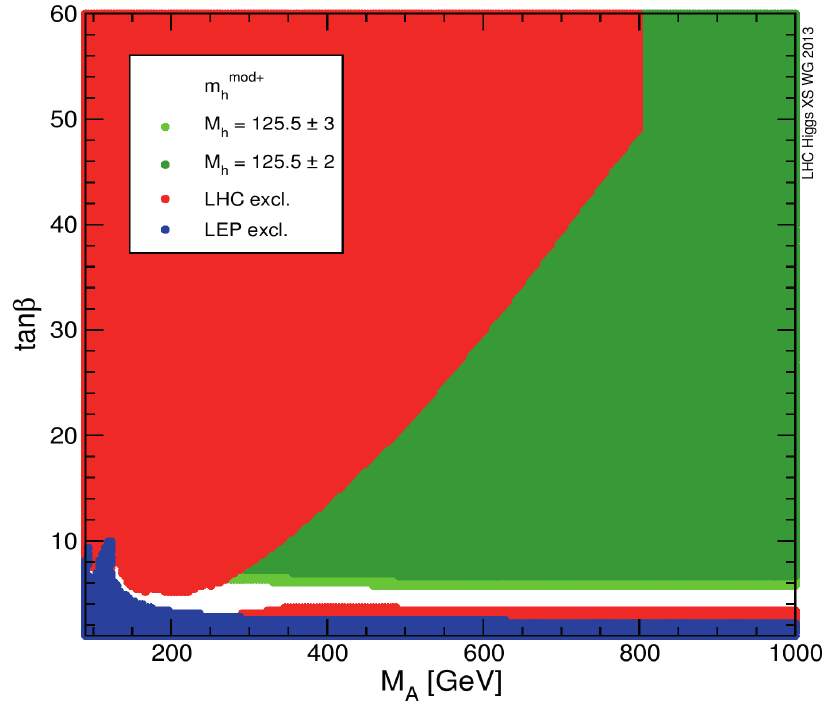
\includegraphics[width=0.6\textwidth]{figure/mh_mod.png}

    \end{center}
    \caption{$m_{A} - \text{tan}\beta$ plane for the  $m_{h}^{mod+}$ scenario, with excluded region
	from direct Higgs searches at Lep (blue) and LHC (red). The two green shades corresponds to
	the allowed parameter space for the assumption of $M_{h} = 125.5 \pm 2 (3)$ GeV. For more detail 
	see~\cite{}.}
   \label{fig:mhmod}
\end{figure}

Under the light of the recent discovery of a Higgs 
boson with mass of 125 GeV \cite{}, remains an open question
wheter this new particle constitute all the pieces of the Higgs
sector or wheter it is only one of several bosons predicted in some theories 
that go beyond the SM. The most recent measurements \cite{} of its
properties shows it to be, within experimental uncertainties, perfectly 
compatible with the SM Higgs boson, however such a new particle can 
be accomodated within several beyond the 
standard model (BSM) theories, this is particularly true for Super Symmetry. 

There are two approach to explore the Higgs sector:
one can study the cupling of the Higgs boson with vector
bosons and fermions, those measure in fact are sensitive to new physics and can determine
%given the unitarity property of scattering
%aplitudes for longitudinal vectors and fermions, one can understand 
if this particle is  fully responsible for
the generation of all the SM particles masses. 
Another approach is to directly search for %model dependent
for additional Higgses in a well defined model, which is the approach followed in this
thesis where new neutral bosons are sought within the MSSM (see chapter \ref{}). 

In the MSSM a Higgs boson with properties that  
resembles the one for a SM Higgs boson occures naturally in large regions 
of parameter space, for practical reason however,
% a point in the MSSM parameter space must now not only pass all the 
%experimental bounds on superparticle masses, but also lead to the prediction of a scalar with
%mass, production cross section and decay rates compatible with those measured at the LHC.
%it is not convenient to scan over a large parameter space as the MSSM has, for practical reason
is usefull to fix  parameter of the model to achieve what is called a benchmark
scenario. With the recent discovery, bechmark scenarios of the MSSM have been updated to fit
with the new constraints (more details on benchmark scenarios are in chapter~\ref{}), 
as an example in figure~\ref{fig:mhmod} are reported the current exclusion limits
for one of those updated scenarios, $m_{h}^{mod+}$, the green area represents what is currently 
allowed in the $m_{A} - \text{tan}\beta$ plane showing that there is still plenty of room for BSM
Higges.

\subsection{How to search for new phenomena?} \label{sec:stat1} 
%\subsection{What is a search?}
In experimental physiscs  an observation of a new phenomena or its exclusion  is 
carachterized by means of statistical statements, in this sense one can say that statistic is the language 
of experimental physics.
Search for new physics at the LHC extesively uses frequentistic statistical tests~\cite{LHCstat}.
%to make
%robust statements about the exsistence or the exclusion of new phenomena, %to make robust statements... qualcosa qui
In this section an itroduction to statistical tests is given, for more details see section~\ref{sec:result}.
 
A \emph{statistical test} is a rule to reject or accept an hypotesis, where for hypotesis is meant 
a statement about the distribution of the data. Typically new physics searches are looking for a signal 
that is additive on top of the background, is then natural to compare two hypotesis:
the background only hypotesis $H_{0}$, or null hypotesis, and the signal plus background hypotesis $H_{1}$, which is the alternative.
In the process of decision making is common to define what is called a \emph{signal region} (SR), which is simply
a set of selections applied to data aimed to enhance signal with respect to the background, 
the observed number of events in the SR, $N_{SR}$,  are used to make probabilistic statements about the two hypotesis.
$N_{SR}$  is in fact a random
variable described by a Poisson distribution, where, in case the null hypotesis is true, $\nu_{B}$ events are expected, otherwise 
in case $H_1$ is true $\nu_{B} + \nu_{S}$ events are expected. The two probability distributions for the two hypotesis
totaly describes the \emph{probability model} for this counting experiment.
%
%the probability model for null and the alternate hypotesis is then respectively 
%$\text{Pois}(N_{SR}|\nu_{B})$ and $\text{Pois}(N_{SR}|\nu_{B} + \nu_{S})$.
Is clear then that the evidence for a signal shows up as an excess of 
events, a way to quantify the conpatibility of the null hypotesis with data
is to make a \emph{significance} test: calculate the probability that 
the background-only would produce at least as many
as the observed events, which is the so called of p-value and in this case is expressed by the formula:
$$
\text{p-value} = \sum_{n=N_{SR}}^{\infty} \text{Pois}(n|\nu_{B})
$$
Calculating  p-values is a way to characterize an excess, in high energy physics the commonly accepted p-value that is
qualified as a discovery is $2.87 \times 10^{-7}$, which is an extremely low probability for the null hypotesis to be true
and corresponds to five standard deviation for a gaussian distribution. 

In case no excess is observed, the procedure is to build a statisctical test where the 
null hypotesis is accepted and at the same time the signal hypotesis
is rejected with a fixed predetermined probability, called confidence level.
A statistical test is a rule that defines a region in the space of data for which
a given hypotesis can be accepted or rejected, often rather than using a full set 
of data $\mathcal{D}$, it is convenient to define a \emph{test statistic}, T, which is usually a single
number computed from the data, the two hypotesis implies different distributions for T, 
then one defines an acceptance region \emph{W} in terms of the test statistic, if 
$T \in W$ the $H_{0}$ is rejected, $H_{1}$ accepted and vice versa,
the probability with which one rejects $H_{1}$ or $H_{0}$ is then given by the choice of
\emph{W} and T. Neuman and Pearson provided a framework for hypotesis testing that addresses the 
choice of the test statistic \cite{NP}.
%such that 
%$P(T \in W | H_{0}) \leq \alpha$, where $\apha$ is the size of the test and correspond to the probability
%for which $H_{0}$ is rejected when is true, 

A discriminating variable is often used to help separating signal and backgrounds, this can be any of the observables of
the experiment, a usually chosen observable is for example the invariant mass of the final state particles. The expected
distributions of this observable for the two hypotesis completes the above
mentioned probability model, the actual implementation is achieved by means of an histograms, 
i.e. by discretizing the distribution of the observable and making a counting experiment
for each bin of the histogram, the resulting probability model is then a product of Poissons: 
\begin{equation}\label{markedpoisson}
\prod_i \text{Pois}(n_i^{observed} ~ | ~ s_i(\vec{\theta}) + b_i(\vec{\theta})) 
\end{equation}
where $s_i$ and $b_i$ are  the number of expected signal and background events in the bin $i$, while $n_i$ are the
actual observed events in the bin $i$. Here is made explicit that the signal and backgrounds expectations
depends also on a set of additional parameter $\vec{\theta}$, called \emph{nuissance parameters}, 
those embed effects like detector mismodeling and theoretical uncertainty.

%A statistical test is a rule that define a region in parameter space for which  a given hypotesis can be accepted or rejected.
%Often rather than using a full set of data $\vec{X}$, it is convenient to define a \emph{test statistic}, t, which is usually a single
%number, it is a quantity calculated out of the data, a mapping of a set of measurements into a single number. The test statistic, that is usually
%connected to the discriminating variable, would then have a different distribution for the different hypotesis, one can then define $\alpha$
%called the size of the test and $t_{\alpha}$ for which $P(t < t_{\alpha} | H_{0}) \leq \alpha$ then in this case $H_{0}$ is rejected.

%- Alternative: NP provided a framework for hypotesis testing that addresses the choice of the test statistic. First one defines 
%an acceptance region in terms of a test statistic, such that if $T(\vec{X}) < t_{\alpha}$ one accepts the null hypotesis. 
%One can think of $T(\vec{X}) = t_{\alpha}$ as a counturn in the space of the data which is the boundary to this acceptance region.
%Then one defines the size of the test $\alpha$ which is the probability for the null hypotesis to be rejected when true,
%the test is totally asymmetric: if the null hypotesis is rejected then the alternate is accepted (is this true??)....

Summarizing, there are several ingredients that constitute a search for new physics:
\begin{itemize}
	\item Definition of a signal region in data where signal is enhanced with respect to the backgrounds, detailed for this analysis in section \ref{sec:topology} 
	and \ref{sec:selectiona}.
	\item Definition of a discriminating variable which is usefull to disentangle between signal and backgrounds, see section \ref{sec:mmc}.
	\item Definition of the probability model, i.e., the expectation for the distribution of the discriminating variable
		 for signal and background hypotesis, this is one of the most importat
		point of a search and main part of the work of this thesis, detailed in section \ref{sec:BackgroundEstimation}.
	\item Definition of a test statistics to quantify an observation or an exclusion, which is discussed for the LHC in section \ref{sec:result}.
\end{itemize}



\subsection{Signal Topology}\label{sec:topology}


This section describes the strategy to enhance the search sensitivity 
taking advantage of the signal topology.
The Sensitivity of a search is the signal strenght that is expected to be  excluded 
in case of no signal. If one is searching for a rare process, then the analysis strategy, i.e. the
plan to enhance the signal sensitivity of the search, is crucial.
This search is complementary to the Standard Model
Higgs search in tau final state, this is also considered in the analysis strategy, 
the focus is then on phase space not explored from SM search.

In the MSSM for large region of parameter space one found that one of the 
$CP$-even neutral Higgses  has properties that resemble the one of the SM Higgs,
this is usually the case for the lightest Higgs, \emph{h}, the other two, $H$ and $A$, 
tend to be degenerate in mass and decouple from gauge bosons.
An interesting fenomenological consequence is that the coupling of the latter
two Higgses with down (up) type fermions are enhanced
(suppressed) by $\tan\beta$, meaning that for large $\tan\beta$
bottom-quark and $\tau$ lepton will play a more important role than in
the SM case either for production and decay.

The production of the neutral $CP$-even MSSM Higgs bosons at hadron
colliders proceeds via the same processes as for the SM Higgs
production. However, the pseudoscalar $A$ instead cannot be produced
in association with gauge bosons or in vector boson fusion (VBF) at
tree-level, as this coupling is forbidden due to $CP$-invariance.  At
the LHC one of the most relevant production mechanisms for the MSSM
Higgs bosons is gluon-gluon fusion, $gg\rightarrow A/H/h$. In
addition, the production in association with $b$-quarks becomes
important for large value of $\tan\beta$. Those are the two production mechanism
that are considered in this analysis, figure~\ref{fig:prod} shows the feyinman-diagram
for those processes, while figure~\ref{fig:xsec} shows the production cross section of the neutral 
MSSM Higgses via these two processes. The search is divided in two category which are optimized
for the two different production mode considered, in the gluon-fusion category
is requred a b-jet veto (for definition of b-tagging algorithm see chapter~\ref{chap:detector}), in fact no b-jet in the final state are present for this
production mode. In contrast a a b-jet tag is required for b-associated production,
this category is expected to be very sensitive to $\tan\beta$. The two category are
ortogonal and present different backgrounds contributions, which can be
optimized separately. 

\begin{figure}[tp]
     \begin{center}

            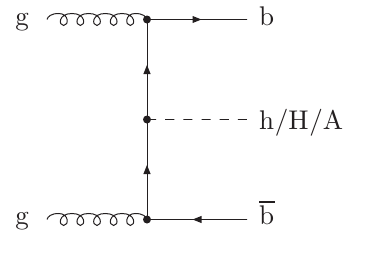
\includegraphics[height=3cm]{figure/bba.png}
            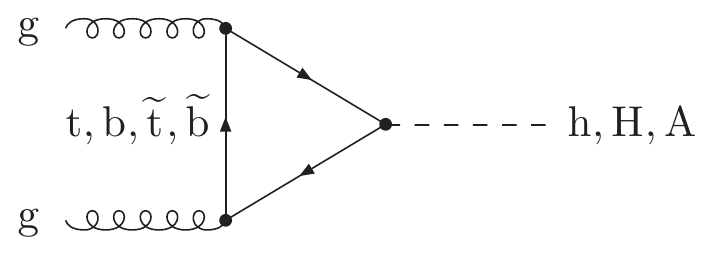
\includegraphics[height=3cm]{figure/ggf.png}

    \end{center}
    \caption{Feynman diagram for b-associated production and gluon-gluon fusion for MSSM neutral Higgs.}
   \label{fig:prod}
\end{figure}

\begin{figure}[tp]
     \begin{center}

            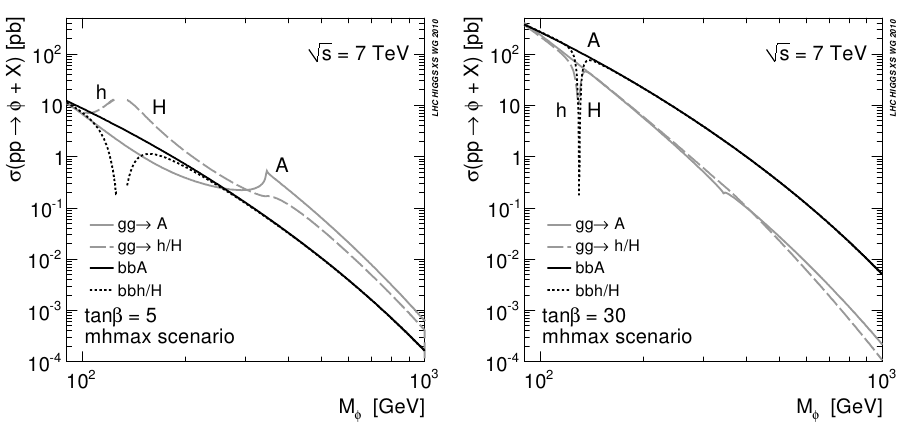
\includegraphics[width=\textwidth]{figure/xsec.png}

    \end{center}
    \caption{Production cross section for the \emph{h/H/A} MSSM neutral Higgs bosons via b-associated production and
	gluon-gluon fusion production mode. The calculation are for the $m_h^{max}$ scenario and for $\tan \beta=5$ (left) and $\tan \beta=30$ (right).}
   \label{fig:xsec}
\end{figure}

\begin{table}[t]
  \begin{center}
   \begin{footnotesize}	
    \begin{tabular}{cc}
      \hline \hline
      Channel & Selection \\
      \hline
      Preselection 	&  Trigger \\
	&	At least one reconstructed vertex \\
	&	Event cleaning	\\
	&	Tau Veto \\
	& 	Exactly one tight isolated electron with $\pt > 15 $ or 25 GeV (trigger dependent) \\
	&	Exactly one Combined isolated muon with  $\pt > 10$ GeV \\
	& 	Opposite charge between the leptons \\ 
      \hline
      b-Tag & Exactly one b-tagged taggable jet \\
      & $\Delta\phi(e-\mu)>2$ \\
      & $\sum\cos\Delta\phi > -0.2$ \\
      & $\sum H_T < 100$ GeV \\
      & $\SumLtMET < 100$ GeV \\
      & Good MMC solution \\
      \hline
      b-Veto & Exactly zero b-tagged taggable jets \\	
      & $\Delta\phi(e-\mu)>1.6$ \\
      & $\sum\cos\Delta\phi > -0.4$ \\
%      & $\SumLtMET < 150 \GeV$ \\
      & Good MMC solution \\
      \hline \hline
    \end{tabular}
    \caption{Summary of the preselection and the full selections used for the b-tag and b-veto channels.}
    \label{tab:sel}
  \end{footnotesize}
  \end{center}
\end{table}

The decays of the neutral
MSSM Higgs bosons (in the assumption that all supersymmetric particle
are heavy enough) are the same as for the SM one with the already
cited exception of $A$. Figure~\ref{fig:xsec} shows the decay branching fractions
for $H$ and $A$ as a function of the mass, 
the decay into tau pair is the most important after $b\bar{b}$ and the one used in this analysis. The 
decay channel in $b\bar{b}$ is in fact very challenging due to the huge background from
QCD multi-jet.
In this thesis only cases in which the taus decay one in $e + 2\nu$ and
the other in $\mu + 2\nu$ are considered, This final state corresponds to a total
$\tau^+\tau^-$ branching ratio of approximately 6\%.
 
%Searches for neutral MSSM Higgs bosons have been performed at
%LEP~\cite{LEPLimits}, the
%Tevatron~\cite{TevatronLimits1,TevatronLimits2,TevatronLimits3,TevatronLimits4,TevatronLimits5,TevatronLimits6}
%and the LHC~\cite{CMSLimit, ATLASLimit}.  In this note a search for
%neutral MSSM Higgs bosons with the ATLAS experiment at CERN is
%presented, using proton-proton collisions at centre-of-mass energy of
%8~TeV, with a recorded integrated luminosity of
%$20.3 \ifb$.

\begin{figure}[tp]
     \begin{center}

            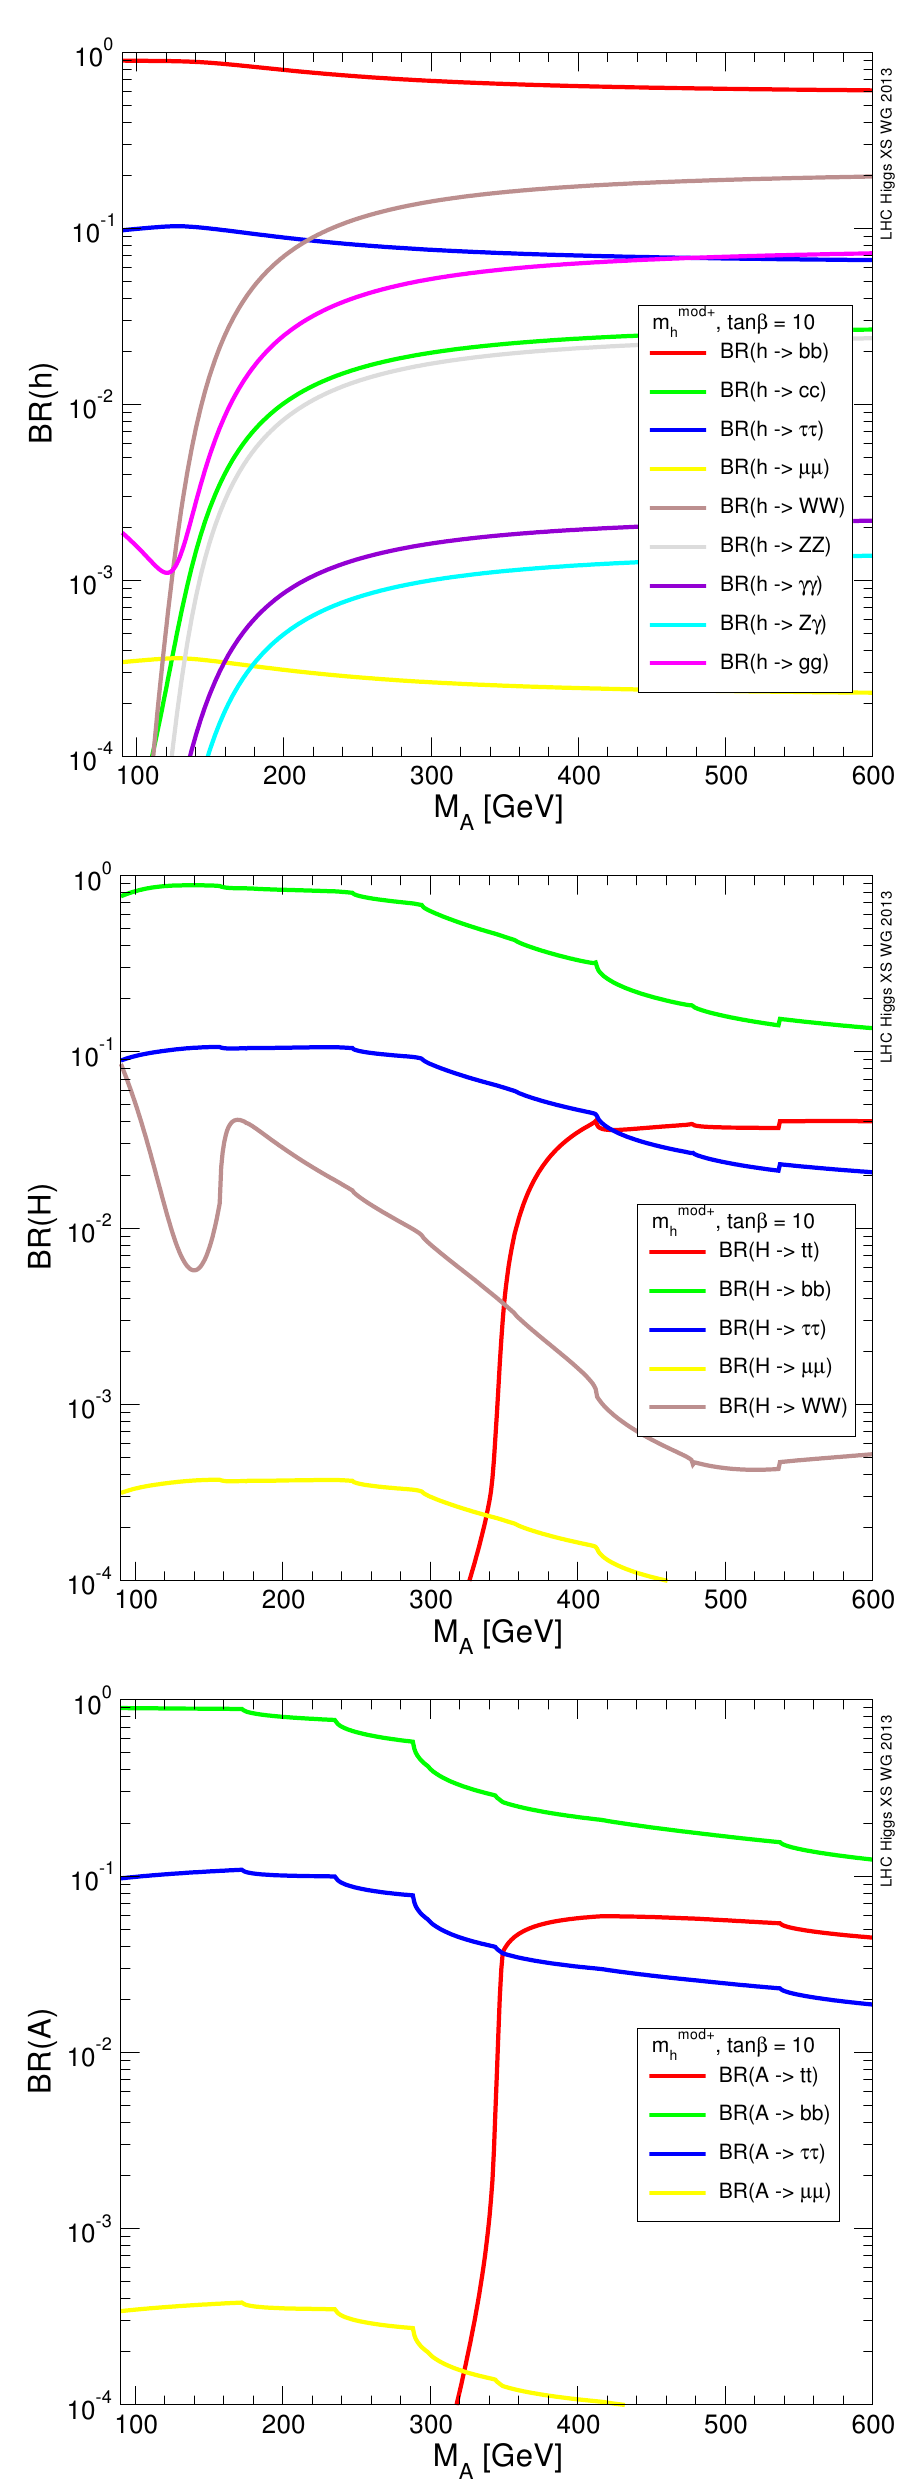
\includegraphics[width=0.5\textwidth]{figure/br.png}

    \end{center}
    \caption{Branching fraction for the MSSM neutral higgses $h/H/A$ in the $m_h^{mod+}$ scenario.}
   \label{fig:br}

\end{figure}


Summarising, the signal topology is characterised by a final state with an
electron, a muon, and missing transverse energy due to the
presence of four neutrinos from the $\tau$ decays. Furthermore, the
final state may be split by the presence or
absence of a $b$-quark initiated jet, depending on the production
process. This signature is achieved experimentally by requiring:
\begin{enumerate}[label=(\roman*)]
\item An OR between an elecron and an electron-muon trigger (\verb=EF_e24vhi_medium1= $||$ \verb=EF_e12Tvh_medium1_mu8=).

\item Exactly one reconstructed electron and one muon of opposite charge, the muon is required to have $\pt > $ 10~GeV, while the electron 
should have $\pt > $ 15 or 25~GeV depending on the trigger that selected the event. For electron and muon object 
definition see chapter~\ref{chap:detector}.

\item The two leptons should be isolated, meaning that in a cone around the lepton there should be little energy deposit (should not be sorraunded by                 
other particle, common of non-promt leptons coming from jets). For more detail about isolation properties see section ~\ref{sec:BackgroundEstimation}.

\item Hadronic $\tau$ veto: the events is rejected if at least one hadronic $\tau$ is found with $\pt > $ 15 GeV.

\item Lepton invariant mass greather than 30 GeV.
\end{enumerate}
This set of selection all togheter are referred in the following as \emph{preselection}. More detail on preselections 
are reported in table~\ref{tab:sel}, for details on object reconstruction and quality requirements see chapter~\ref{chapted:detector}. 
The two analysis category, \emph{b-tag} and \emph{b-veto}, are defined adding on top of the preselections 
the request of "exactly one b-tagged jet" or "no b-tagged jet" in the event respectively, to be 
\emph{taggable} a jet should have $\pt > 20$ GeV and $|\eta| < 2.5$.


\subsection{How to deal with Backgrounds}\label{sec:selectiona}
%\subsection{Selections}
The signal topology described in the previous section is common to many other processes, unfortunately, 
those have higher cross section than the sought signal and a set of additional selections
is needed to enhance the sensitivity of the search.
The most important backgrounds to this search are the production of
 $\Ztautau $ + jets, the top quark ($t\bar{t}$ and single top production is intended), diboson production 
(like $WW$ or $ZZ$ events) and Drell-Yan process or events with non-prompt leptons coming 
solely from hadron decay (in short QCD multi-jet).
Vector bosons production like  $\Wlnu$ or $\Zll$ + jets (with $\ell$ here meaning either $e$ or $\mu$) are also considered,
however those processes have a limited impact.

The final state of Higgs decaying into tau pair coincide with the one from  $\Ztautau$  process, this is then an irreducible 
background. Exploiting the different kinematics of the Higgs decay with respect to other backgrounds it possible to disentangle
between the two. In the Higgs decaying into $\tau^{+} \tau^{-} \rightarrow e ~ \mu + 4\nu$ the taus are highly boosted
and this feature is transferred to the final state leptons, their kinematics then result to be  significantly different 
with respect to process like diboson or $\ttbar$. A first difference is that  $e$ and $\mu$ from the Higgs decay will be more likely "back-to-back",
as it is shown in Figure~\ref{dphi} where the angle between the leptons in the transverse plane $\Delta\phi = |\phi_{e} - \phi_{\mu}|$ 
is reported.  Furthermore the neutrinos will be more likely collinear with the charged leptons:
this feature can be matematically seen as the sum of scalar product between missing energy and the leptons four-vectors in the
transverse plane, if the vectors are normalised to unit versors then what remains is a relation only between angles:
$$ \hat{E}_{T}^{miss} \cdot ( \hat{P}_{T}^{\mu} + \hat{P}_{T}^{e} ) = cos(\Delta\phi_{E_{T},\mu}) + cos(\Delta\phi_{E_{T},e}) = \sum_\ell cos(\Delta\phi_{E_{T},\ell}) $$
collinearity implies this sum to be equal to zero as it is shown in figure~\ref{sumcosphi}. 
These two feature can be used to distinguish between mu-e coming from decay from highly 
boosted object and the one coming from W decays in top or in dibosons backgrounds which will have a more spread distribution.
In b-veto category these two variables are sufficient to suppress contribution from dibosons,
no other selection is applied in this category because it has been shown to not bring significant improvement.

In the b-tag category the situation is different, 
the  request of b-jet enhance backgrounds with high jet activity as top production, given the relatively low
jet activity of Higgs events (also in the case of b-associated production) it is possible to separate them from
top production which instead is very likely to have two or more highly enegetic jets in the event.
Little jet activity is achieved by requesting requesting the sum of the jets $\pt$ in the event to be small, this variable is called $\Ht$
and is shown in figure~\ref{Ht}.
Another feature that distinguish top pair production from Higgs is the much higher invariant mass of the former final state,
in the transverse plane all the leptons will tend to have a higher momentum, the sum of lepton \pt and \met is then used as
a discriminating variable. Figure~\ref{sumlepPt} shows the distribution of this last analysis variable.

The above described variables defines the signal region in the b-tag and b-veto category,
in table~\ref{tab:sel} a summary of the preselection and all the selection variable used with their optimized cut values is reported.
Figure~\ref{fig:mass} shows the final state invariant mass distribution (here the \mmc 
discriminating variable is used see section~\ref{sec:mmc}) as a function of the selection stage,
while in tables~\ref{tab:eventsel:bveto}-\ref{tab:eventsel:btag} the number of events that survises at each cut stage for different background is reported.

\begin{figure}[p]
     \begin{center}
     \subfigure[]{		
            \includegraphics[page=11,width=0.47\textwidth]{figure/std_plots_presel.pdf}
	    \label{dphi}	
     }	
     \subfigure[]{		
            \includegraphics[page=12,width=0.47\textwidth]{figure/std_plots_presel.pdf}
	    \label{sumcosphi}	
     }	
     \subfigure[]{		
            \includegraphics[page=9,width=0.47\textwidth]{figure/std_plots_presel.pdf}
	    \label{Ht}	
     }	
     \subfigure[]{		
            \includegraphics[page=10,width=0.47\textwidth]{figure/std_plots_presel.pdf}
	    \label{sumlepPt}	
     }	

    \end{center}
    \caption{Distribution of analysis variable after preselection.}
   \label{fig:selections}
\end{figure}


\subsection{Mass Reconstruction with MMC Technique}\label{sec:mmc}

Reconstructing the invariant mass of a di-tau system from the tau decay products is a challenging task
due to the presence of neutrinos in the final state. 
In a di-tau system in which both taus decays leptonically (with a total of four neutrinos) there are eight uknowns, those are the components of the two 
four-vectors that represents the missing momentum (carried out by neutrinos) in each tau decay. There are four additional constraint 
which come from the measures of \MET and from the fact that each single decay should have invariant mass equal to the tau mass,
therefore there are still four degrees of freedom in the system.
Several approximation are possible to further constraint the momentum carried by neutrinos,
for example assuming them collinear to the other leptons from tau decay, however those approximation suffers of limitations. 

In this analysis, the so-called "Missing Mass Calculator" (MMC)~\cite{MMC}
is used to calculate the di-tau system invariant mass from its decay products and the \met. This technique employs additional 
information from the well known tau decay to constraint the system:
in the above mentioned four dimensional parameter space, in which lies the solution of the di-tau system, not all the points are 
equally likely for a given event topology, using Pythia simulation supplemented with TAUOLA package,
a likelihood based on $\Delta R  =  \sqrt{\Delta\eta^2 + \Delta\phi^2}$ distribution between the missing energy and each of the two "visible" leptons is build, 
minimising the likelihood for a given event topology it is possible to determine the most likely point in the parameter space
and solve the system. Effect of resolution are taken into account by producing a mass distribution
for each of the scanned points in the parameter space. As a result this method give a more precise measurement of the di-tau
system invariant mass and a considerable improvement in resolution. The invariant mass distribution 
calculated with the MMC technique is referred in the following as $\mmc$ and is used as discriminating 
variable in the limits setting.


 
%Accurate invariant mass reconstruction of a di-tau system is a challenging task due to the escaping neutrinos.
%In this analysis, with four neutrinos in the final state, the number of unknown largely exceed the number of constraints,
%several approximation are possible to further constraint the neutrinos, for example assuming them collinear to the 
%other leptons from tau decay, however those approximation suffers of limitations. 

%In this analysis we use the so called missing mass calculator (MMC)~\cite{MMC}
%technique for the calculation of the di-tau system invariant mass. This technique employs additional 
%information from the well known tau decay to constraint the system, this is achieved by minimising a likelihood function 
%defined in the kinematically allowed phase space region, the result is a more precise measurement of the di-tau 
%system invariant mass and a considerable improvement in resolution. The invariant mass distribution 
%calculated with the MMC technique is referred in the following as $\mmc$ and is used as discriminating 
%variable in the limits setting.

\begin{figure}[p]
     \begin{center}
     
     \subfigure[]{		
            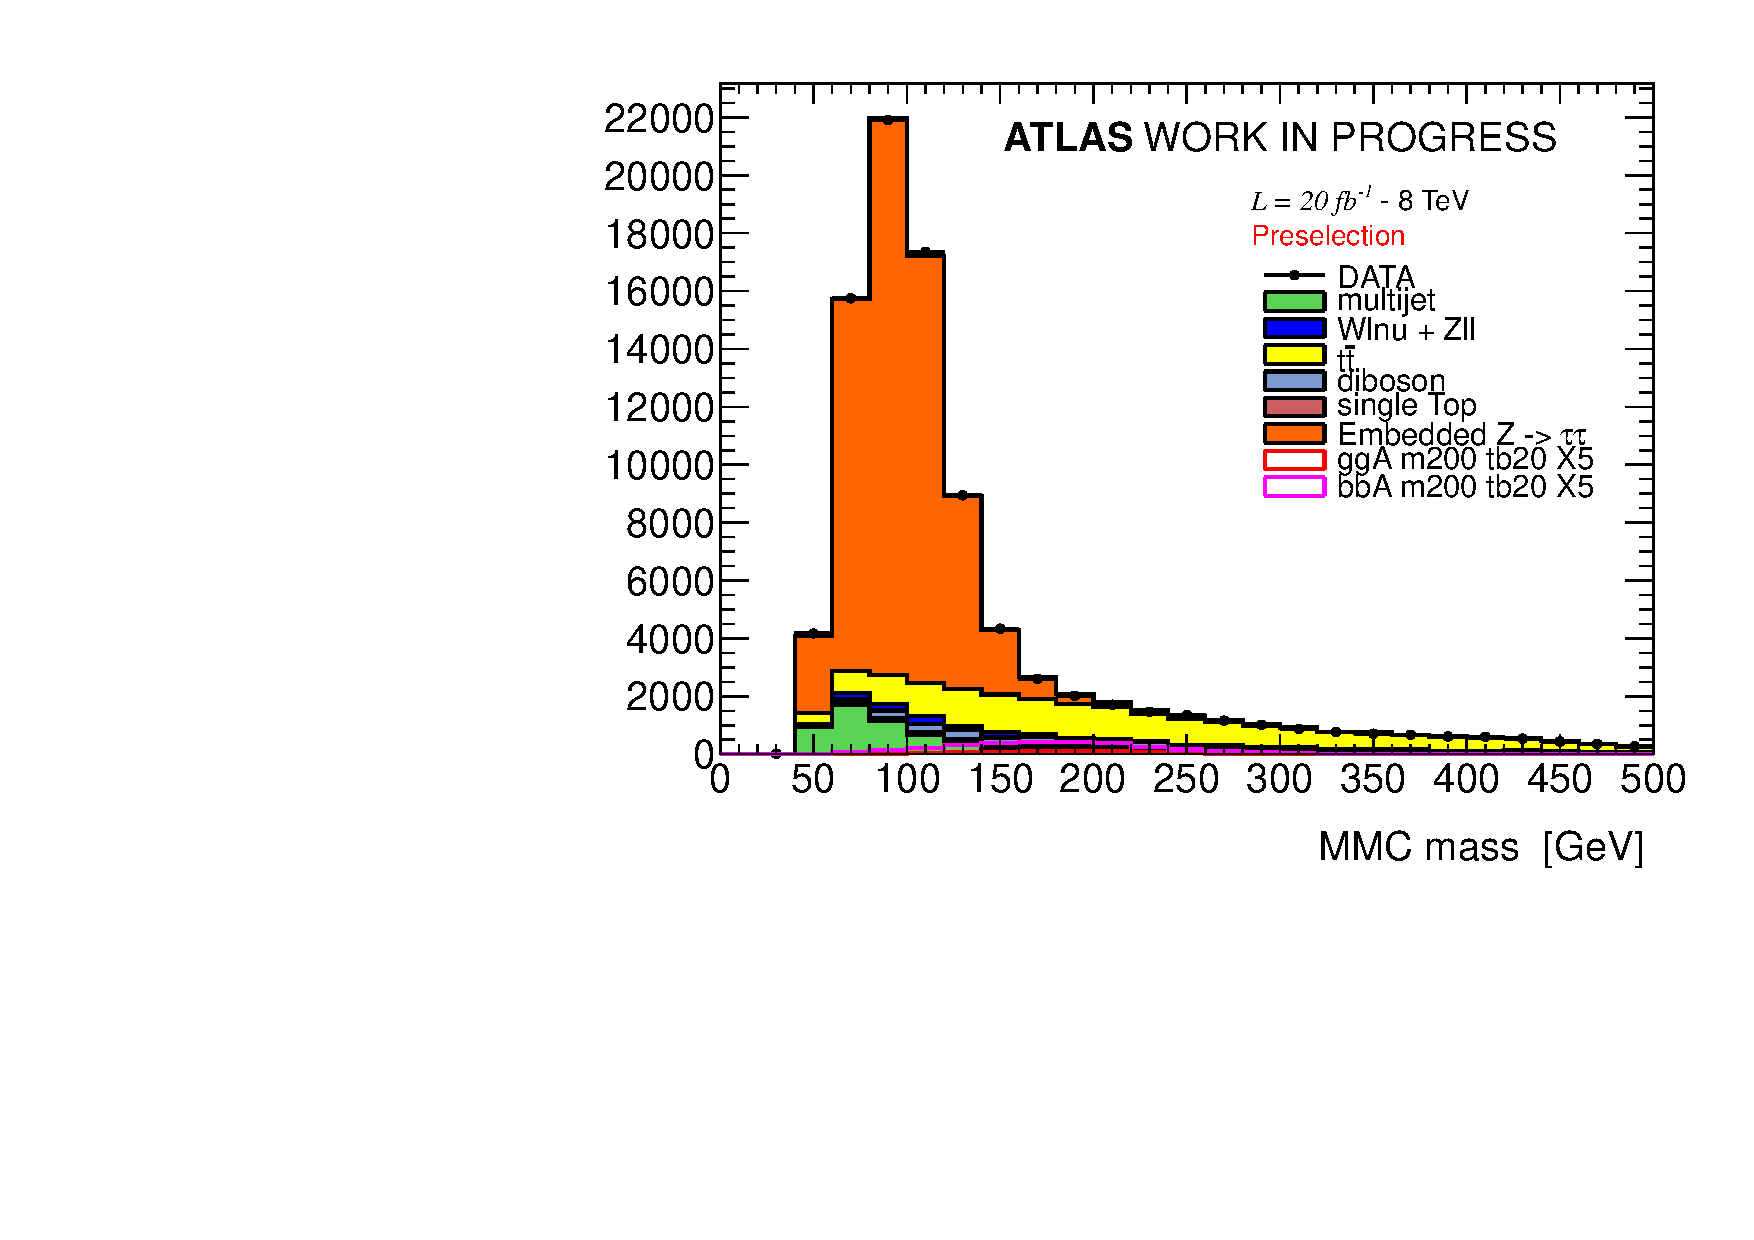
\includegraphics[page=1,width=0.47\textwidth]{figure/std_plots_mass.pdf}
	    \label{presel}	
    	%\caption{\footnotesize Preselection.}
     }\\	
    \end{center}

     \subfigure[]{		
            \includegraphics[page=3,width=0.47\textwidth]{figure/std_plots_mass.pdf}
	    \label{veto}	
    	%\caption{\footnotesize B-veto.}
     }	
     \subfigure[]{		
            \includegraphics[page=2,width=0.47\textwidth]{figure/std_plots_mass.pdf}
	    \label{tag}	
    	%\caption{\footnotesize B-tag.}
     }	
     \subfigure[]{		
            \includegraphics[page=5,width=0.47\textwidth]{figure/std_plots_mass.pdf}
	    \label{fullveto}	
    	%\caption{\footnotesize full B-veto.}
     }	
     \subfigure[]{		
            \includegraphics[page=7,width=0.47\textwidth]{figure/std_plots_mass.pdf}
	    \label{btagphi}	
    	%\caption{\footnotesize B-tag + $\Delta\phi$ + $\sum_\ell cos(\Delta\phi_{E_{T},\ell})$.}
     }
     
     \subfigure[]{		
            \includegraphics[page=6,width=0.47\textwidth]{figure/std_plots_mass.pdf}
	    \label{fullbtag}	
    	%\caption{\footnotesize full B-tag.}
     }
     	

    \caption{\footnotesize Distribution of the \mmc for different cuts stage, see text. Left column corresponds to b-tag category, right column to b-veto.}
   \label{fig:mass}
\end{figure}



\begin{sidewaystable}
  \centering
   \begin{footnotesize}	
  \begin{tabular}{ccccccccc}
    \hline\hline
	& Preselection			&	n(b-jet)=1			&	$\Delta\phi(e-\mu)>2$			&	$\sum\cos\Delta\phi > -0.2$			&	$\SumLtMET < 100 $ GeV			&	$\sum H_T < 100$ GeV			&	mmc			\\
   \hline
Data	&	125886			&	23352			&	-			&	-			&	-			&	-			&	-			\\
Multijet	&	6700	$\pm$	500	&	330	$\pm$	40	&	208	$\pm$	27	&	135	$\pm$	22	&	114	$\pm$	17	&	100	$\pm$	15	&	100	$\pm$	15	\\
\Zll 	&	570	$\pm$	50	&	5.2	$\pm$	1.8	&	2.3	$\pm$	1.1	&	2.3	$\pm$	1.1	&	1.7	$\pm$	1.0	&	0.9	$\pm$	0.8	&	0.9	$\pm$	0.8	\\
\Wlnu	&	1630	$\pm$	150	&	20	$\pm$	6	&	15	$\pm$	6	&	13	$\pm$	6	&	10	$\pm$	6	&	10	$\pm$	6	&	10	$\pm$	6	\\
Diboson	&	9340	$\pm$	50	&	99	$\pm$	5	&	63	$\pm$	4	&	36.4	$\pm$	3.0	&	14.8	$\pm$	1.8	&	13.3	$\pm$	1.8	&	13.1	$\pm$	1.8	\\
\ttbar	&	40630	$\pm$	110	&	19810	$\pm$	70	&	9680	$\pm$	50	&	6450	$\pm$	50	&	808	$\pm$	15	&	350	$\pm$	10	&	330	$\pm$	10	\\
Single Top	&	4450	$\pm$	40	&	2456	$\pm$	33	&	1223	$\pm$	23	&	784	$\pm$	18	&	122	$\pm$	7	&	99	$\pm$	7	&	90	$\pm$	6	\\
\Ztautau	&	61500	$\pm$	70	&	952	$\pm$	9	&	625	$\pm$	7	&	540	$\pm$	7	&	482	$\pm$	6	&	421	$\pm$	6	&	418	$\pm$	6	\\
Signal	&				&				&	-			&	-			&	-			&	-			&	-			\\
    \hline
    \hline
  \end{tabular}
  \caption{Number of data and background events in the b-tag channel.}
  \label{tab:eventsel:btag}
   \end{footnotesize}	
\end{sidewaystable}


%\begin{sidewaystable}
%  \centering
%  \begin{tabular}{ccccccccc}
%    \hline\hline
%   & Data & \Ztautau & \Zll &  \Wln & Single Top & \ttbar & Dibosons & Multi-jet \\
%   \hline
%Preselection & 188421	&79175.7 $\pm$	253.9	&853.4 $\pm$	66.6	&4977.5 $\pm$	387.3	&5265.5 $\pm$	48.9	&58575.1 $\pm$	175.7	&10726.5 $\pm$	51.3	&33831.6 $\pm$$\pm$	742.7 \\
%Exactly zero b-tagged jets & -	&78397.4 $\pm$	253.5	&840.3 $\pm$	66.2	&4905.7 $\pm$	386.8	&2235.2 $\pm$	34.3	&13313.3 $\pm$	93.9	        &10590.6 $\pm$	51.0	&31916.2 $\pm$	721.7 \\
%$\Delta\phi(e-\mu)>1.6$  & -	&75551.4 $\pm$	252.1	&725.2 $\pm$	62.7	&3503.7 $\pm$	307.8	&1492.3 $\pm$	27.9	&8465.6 $\pm$	73.1	        & 8387.3	$\pm$ 45.4 	&28831.1 $\pm$	594.7 \\
%$\sum\cos\Delta\phi > -0.4$ &-	&72161.7 $\pm$	249.8	&632.5 $\pm$	59.6	&2112.2 $\pm$	202.7	&925.1 $\pm$	22.5	&5635.9 $\pm$	59.0	        & 4535.9 $\pm$	33.3	        &23625.5 $\pm$	413.3 \\
%  \hline
%    \hline
%  \end{tabular}
%  \caption{Number of data and background events in the b-veto channel.}
%  \label{tab:eventsel:bveto}
%\end{sidewaystable}

\begin{table}
  \centering
   \begin{footnotesize}	
  \begin{tabular}{cccccc}
    \hline\hline
	&	Preselection			&	n(b-jet)=0			&	$\Delta\phi(e-\mu)>1.6$			&	$\sum\cos\Delta\phi > -0.4$ 			&	mmc			\\
    \hline
   \hline
Data	&	125886			&	89155			&	-			&	-			&	-			\\
Multijet	&	6693	$\pm$	456	&	6357	$\pm$	461	&	5322	$\pm$	438	&	4137	$\pm$	339	&	3934	$\pm$	335	\\
\Zll 	&	569	$\pm$	48	&	564	$\pm$	48	&	516	$\pm$	47	&	434	$\pm$	44	&	432	$\pm$	44	\\
\Wlnu	&	1625	$\pm$	155	&	1604	$\pm$	155	&	1145	$\pm$	125	&	714	$\pm$	101	&	656	$\pm$	100	\\
Diboson	&	9338	$\pm$	48	&	9235	$\pm$	48	&	7358	$\pm$	43	&	4002	$\pm$	31	&	2925	$\pm$	27	\\
\ttbar	&	40632	$\pm$	106	&	7707	$\pm$	46	&	5044	$\pm$	37	&	3416	$\pm$	31	&	2159	$\pm$	24	\\
Single Top	&	4449	$\pm$	44	&	1664	$\pm$	27	&	1124	$\pm$	22	&	682	$\pm$	18	&	435	$\pm$	14	\\
\Ztautau	&	61503	$\pm$	68	&	60440	$\pm$	67	&	58078	$\pm$	65	&	55303	$\pm$	64	&	54683	$\pm$	63	\\
Signal	&				&				&	-			&	-			&	-			\\
    \hline
  \end{tabular}
  \caption{Number of data and background events in the b-veto channel.}
  \label{tab:eventsel:bveto}
   \end{footnotesize}	
\end{table}
